\subsection{Situations} % Change title
Using probability theory, we can calculate the chances of events given the distribution. While the type of distribution can often be inferred, finding the hidden parameter is a very challenging task.


\subsection{Philosophy}
Bayesian inference is based around the idea that one never encounters a situation without previous knowledge! For example, you may know, that the dice is likely fair, and otherwise, probably loaded in favor of higher numbers. This information is as valuable as any other, and should be combined with your new observations. Using this, we can calculate the chances of you rolling quintuple sixes... \textbf{given} your previous knowledge, and the fact you have already rolled quadruple sixes. This is achieved by not considering the probabilities as constants, but as random variables themselves.

\subsection{Prior distribution}
\begin{definition}
	Let \(X\) be a random variable with a distribution depending on the outcome \(\theta \) of the random variable \(\Theta \). The distribution of \(\Theta \) is called the \textit{prior} distribution, while the distribution of \(X|\Theta \) is called the data distribution.

	The prior distribution represents your prior knowledge of the parameter, while the data distribution represents the distribution of \(X\) given you know the outcome of \(\Theta \) which the distribution depends on. 
\end{definition}

\begin{example}
	Let the result of a coin flip (0 if tails, 1 if heads) be \(X|\Theta \sim \operatorname{Ber}(\theta )\) where \(\theta\) is the chance of flipping heads. When seeing a new coin its properties affect the chances of flipping heads, and might be distributed as \(\Theta \sim \operatorname{Beta}(2, 2)\). The former is the data distribution, the latter the prior distribution.
\end{example}

\begin{obs}
	Most further calculations will be done only in the continuous case, the discrete case is left as an exercise.
\end{obs}


\begin{definition}[Prior predictive distribution]
	The distribution of \(X\) is the called the prior predictive distribution. It is what we, before observing more data, would find to be the distribution of \(X\). It is calculated from our prior distribution and data distribution, as the marginal distribution of the simultaneous distribution 
	\[
		f_{X, \Theta }(x,\theta) = f_\Theta(\theta )  \cdot f _{X|\Theta }(x|\theta ).
	\]
	That is,
	\[
		f_X(x) = \int_{-\infty }^{\infty} f_\Theta(\theta )  \cdot f _{X|\Theta }(x|\theta ) d \theta 
	\]
	
\end{definition}


\subsection{Posterior distribution}
The goal of Bayesian inference is creating the posterior distribution \(\Theta | X=x \) where \(x \) is an outcome of the random variable \(X\). That is, using the previous outcomes, we update our belief of what the distribution of \(\Theta \) may be.

\begin{definition}[Posterior distribution] % Adjust to allow for more outcomes
	The posterior distribution \(\Theta |x\) is defined as
	\[
		f _{\Theta |X}(\theta |x) = \frac{f _{X|\Theta}(x|\theta )  \cdot f_\Theta (\theta )}{f_X(x)} 
	\]
	and is simply an application of Bayes' rule!!!
\end{definition}

\begin{obs}
	Once we have calculated the posterior distribution, we may calculate anything we would ever want to know about the distribution of \(X\).
\end{obs}

\begin{obs}
	The gamma function is defined as 
	\[
		\Gamma(x) = \int_{0}^{\infty} t^{x-1} \cdot e^{-t}dt
	\]
	and has the property \(\Gamma(x)  \cdot x = \Gamma(x+1)\) 
\end{obs}


\begin{example}
	Let \(\Theta \sim \operatorname{Gamma}(\alpha , \lambda)\) (the prior distribution) and \(X \sim \operatorname{Exp}(\theta) \) (the data distribution). The density functions become
	\begin{align*}
		f _{\Theta}(\theta) &= \frac{\lambda ^ \alpha }{\Gamma (\alpha )} \theta ^{\alpha -1} e ^{-\lambda \theta } \\
		f _{X | \Theta }(x | \theta ) &= \theta e ^{-\theta x}
	\end{align*}
	where \(\theta , x > 0\).

	The prior predictive distribution becomes
	\begin{align*}
		f _{X }(x) &= \int_{0}^{\infty} f _{x, \Theta }(x, \theta) d \theta \\
							 &= \int_{0}^{\infty} f _{\Theta }(\theta ) f _{X | \Theta }(x | \Theta ) d \theta \\
							 &= \int_{0}^{\infty} \frac{\lambda ^ \alpha }{\Gamma (\alpha )} \theta ^{\alpha -1} e ^{-\lambda \theta }  \cdot \theta e ^{-\theta x} \\
							 & = \frac{\lambda ^ \alpha }{\Gamma (\alpha )} \int_{0}^{\infty} \theta ^{\alpha } e ^{- \theta (x + \lambda )}d \theta \\ 
							 & = \frac{\lambda ^ \alpha }{\Gamma (\alpha )} (\lambda +x ) ^{- \alpha -1} \int_{0}^{\infty} u ^{\alpha } e ^{- u}du \\
							 & = \frac{\lambda ^ \alpha }{\Gamma (\alpha )} (\lambda +x ) ^{- \alpha -1} \Gamma(\alpha+1) \\
							 & = \alpha \lambda ^ \alpha  (\lambda +x ) ^{- \alpha -1}
	\end{align*}

	We may then calculate the posterior distribution
	\begin{align*}
		f _{\Theta |X}(x | \theta ) &= \frac{ f _{x, \Theta }(x, \theta) }{f _X (x)} \\
																&= \frac{f _{\Theta }(\theta ) f _{X | \Theta }(x | \Theta ) }{f _{X}(x)}  \\
																&= \frac{\frac{\lambda ^ \alpha }{\Gamma (\alpha )} \theta ^{\alpha -1} e ^{-\lambda \theta }  \cdot \theta e ^{-\theta x}}{\alpha \lambda ^ \alpha  (\lambda +x ) ^{- \alpha -1}} \\
																&= \frac{(\lambda + x)^{\alpha +1}}{\Gamma(\alpha ) \alpha } \theta ^{\alpha} e ^{\theta (\lambda +x)}\\
																&= \frac{(\lambda + x)^{\alpha +1}}{\Gamma(\alpha +1)} \theta ^{\alpha + 1 -1} e ^{\theta (\lambda +x)}
	\end{align*}
	Which we can easily recognise as the gamma distribution, giving us
	\[
		\Theta | X \sim \operatorname{Gamma}(\alpha +1, \lambda + x)  
	\]

	
\end{example}

\begin{definition}[Proportionality]
	A function \(f(x)\) is proportional to a function \(g(x)\) if there is a constant \(c \ne 0\) such that for all \(x\), 
	\[
		f(x) = c  \cdot g(x).
	\]

	We write this relationship
	\[
		f(x) \propto g(x).
	\]
	If they are dependent on multiple variables, the relevant one will be given by the context.
\end{definition}


\begin{example}
	Let \(\Theta \sim \operatorname{Beta} (\alpha , \beta )\) and \(X|\Theta \sim \operatorname{Bin}(n, \theta)\). The density functions will then be
	\begin{align*}
		f_ \Theta (\theta ) &= \frac{\Gamma(\alpha + \beta) }{\Gamma(\alpha )\Gamma(\beta )} \theta ^{\alpha -1} \theta ^{\beta -1} \\
		f _{X | \Theta }(x | \theta ) &= \binom{n}{x} \theta ^x (1-\theta ) ^{n-x} \\
	\end{align*}
	We notice that in respect to \(\theta \) the posterior distribution is proportional to
	\begin{align*}
		f _{\Theta |X}(\theta | x) 
			&= \frac{ f _{x, \Theta }(x, \theta) }{f _X (x)} \\
			&= f _{x, \Theta }(x, \theta) \\
			&= f _{x| \Theta }(x| \theta)  \cdot f _{\Theta } (\theta )\\
			&\propto \theta ^x (1-\theta ) ^{n-x}  \cdot \theta ^{\alpha -1} \theta ^{\beta -1} \\
			&= \theta ^{\alpha + x - 1} (1 - \theta ) ^{\beta + n - x - 1}. \\
	\end{align*}
	We notice that this is proportional to the beta distribution. As the integral of the function is 1, we can then scale the function to satisfy the criterion. We may otherwise notice this is a scaled version of the Beta distribution and scale it to match, giving us
	\[
		\Theta |X \sim \operatorname{Beta} (\alpha +x, \beta + n -x).
	\]
\end{example}


\begin{obs}
	Notice that this rule may be used to update the distribution multiple times. These updating rules can often be found in formula sheets, but are derived as above.
\end{obs}

\begin{example}
	Let \(\Theta \sim \operatorname{Beta} (2, 2)\) and \(X|\Theta \sim Ber(\theta)\). For example \(X\) could be \(1\) if we flip heads, and \(1\) if we flip heads. While flipping 5 heads in a row, and updating each time, we notice our distribution gets heavily skewed towards higher probabilities of heads.
	\begin{figure}[H]
		\centering
		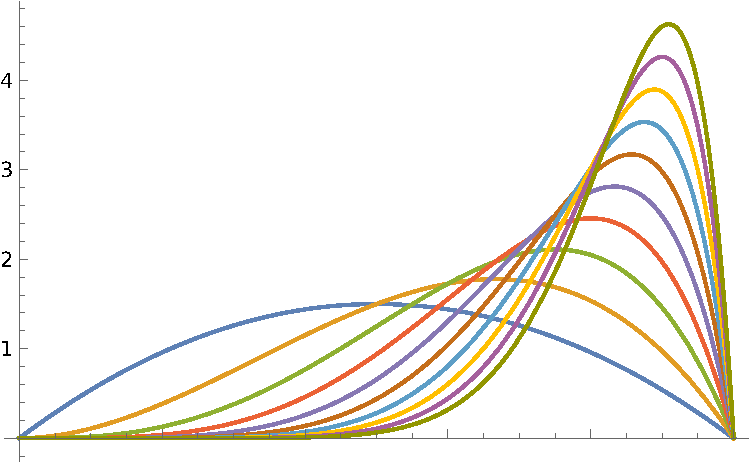
\includegraphics[width=0.5\textwidth]{beta.pdf}
	\end{figure}
	If our prior distribution had been less varied, the results would have been showing later.
\end{example}

\subsection{Exercise problems}

\begin{problem}
	Find the updating rule for \(X | \Theta  \sim \operatorname{Po} (\theta)\) and \(\Theta \sim \operatorname{Gamma} (\alpha, \lambda )\) where
	\[
		f _{X|\Theta }(x|\theta ) = \frac{e ^{- \lambda} \lambda ^x}{x!}.
	\]
\end{problem}

\begin{problem}
	Find the updating rule for \(\Theta \sim N(\mu , \sigma _1^2)\) and \(X | \Theta \sim N(\theta , \sigma _2^2 \) where the \(N(\mu , \sigma \) is the normal distribution with density function
	\[
		\frac{1}{\sqrt{2 \pi \sigma ^2} } e ^{- \frac{(x-\mu) }{2 \sigma ^2} }.
	\]
	Find the updating rule!
\end{problem}

\begin{problem}
	Given the posterior distribution, how would you find an interval where \(\Theta \) has \(p\) probability to be within it?
\end{problem}

\begin{problem}
	If you have the posterior distribution, and the data distribution. How could you calculate the posterior predictive distribution?
\end{problem}
